% ASRN: Adaptive Sparse Recurrence Network -- preprint para Zenodo (version en espanol)
% Autor: Alexis Calvario. Texto y figuras: CC BY 4.0. Codigo: Apache 2.0.
% Compilar: latexmk -pdf ASRN_Calvario_2026_es.tex   (figuras: python paper/hacer_figuras.py)
% Numeros: results/banco_a100, results/citas, results/citas_a100 (ASRN 1.0) y, solo como replicacion,
% history/results/banco_a100_pt211. docs/TECHNICAL_REPORT_es.md es la version larga de este preprint.
\documentclass[11pt]{article}
\usepackage[utf8]{inputenc}
\usepackage[T1]{fontenc}
\usepackage[spanish,es-noshorthands,es-tabla]{babel}
\usepackage{lmodern}
\usepackage[margin=1in]{geometry}
\usepackage{amsmath,amssymb,amsthm}
\usepackage{graphicx}
\usepackage{booktabs}
\usepackage{xcolor}
\usepackage[numbers,sort&compress]{natbib}
\usepackage{microtype}
\usepackage{caption}
\usepackage{enumitem}
\usepackage[hidelinks]{hyperref}

\captionsetup{font=small,labelfont=bf}
\setlist{itemsep=2pt,topsep=4pt}
\graphicspath{{figuras/es/}}
\decimalpoint

% DOI de Zenodo: se llena despues de reservarlo en Zenodo ("Reserve DOI"); vacio, no se imprime.
\def\zenododoi{}

\newcommand{\B}{B}
\newcommand{\Nset}{\mathcal{N}}
\DeclareMathOperator{\softplus}{softplus}
\DeclareMathOperator{\LN}{LN}
\DeclareMathOperator{\GELU}{GELU}
\DeclareMathOperator{\softmax}{softmax}

\title{\textbf{ASRN: Redes de Recurrencia Dispersa Adaptativa}\\[4pt]
\large Copia a larga distancia con memoria lineal, un reloj de tiempo propio aprendido\\ y una puerta de copia
guiada por un proceso de Hawkes}
\author{Alexis Calvario\\ \small Investigador independiente\\ \small ORCID: \href{https://orcid.org/0009-0004-0854-6398}{0009-0004-0854-6398}}
\date{\small Preprint, versión 1.0 --- octubre de 2026%
\ifx\zenododoi\empty\else\\ DOI: \href{https://doi.org/\zenododoi}{\zenododoi}\fi}

\begin{document}
\maketitle

\begin{abstract}
\noindent El trabajo por pieza de la atención crece con el contexto, mientras que los modelos de tiempo lineal como
Mamba-2 y RWKV-7 mantienen un estado de tamaño fijo y pierden la recuperación exacta de trozos lejanos. ASRN (Adaptive
Sparse Recurrence Network, red de recurrencia dispersa adaptativa) es una capa de modelo de lenguaje que recupera
apariciones anteriores exactas con trabajo acotado por pieza: cada pieza atiende solo a sus $C$ compañeros más recientes
en casilleros de hash de signo aprendidos y copia la pieza que \emph{vino después} de cada coincidencia; un \emph{reloj
de tiempo propio} aprendido, $B_t=\sum_{u\le t}\beta_u$, fija el olvido $\alpha_s e^{-\kappa(B_t-B_s)}$ tanto de los
puntajes de recuperación como de una intensidad autoexcitada (de Hawkes) sobre grupos de $n$ piezas repetidos; y una
puerta lee esas intensidades y una racha de repetición mediante una respuesta \emph{no monótona} aprendida para decidir
cuándo copiar. La versión 1.0 agrega a la capa de v89 protecciones numéricas (máscara exacta, un reloj de 64 bits,
topes) que cierran una fuga causal y una deriva del reloj medidas, a cambio de +7.5\% de tiempo y +5.2\% de memoria con
262k piezas, y escribe en tiempo $O(1)$ por pieza nueva. En una A100, con 262{,}144 piezas una capa ASRN es 21.6$\times$
más rápida que la atención con FlashAttention-2, 7.6$\times$ más rápida que RWKV-7 y 2.5$\times$ más rápida que un
bloque de Mamba-2 sin \texttt{causal-conv1d}; un modelo de $\approx$50M parámetros entrena a 163--172k piezas/s de 1k a
32k piezas por secuencia (199--210k compilado), 2.08$\times$ la velocidad de nuestro Transformer++ con 32k (2.20$\times$
con ambos compilados), que es más rápido por debajo de unas 2.4k piezas (5.4k compilados). Con 2.5--46M parámetros y 3
semillas, ASRN copia con 4$\times$ el largo de entrenamiento cuando sale de la meseta inicial (99.99\% y 99.98\%; la
tercera semilla se quedó en ella), mantiene la recuperación en MQAR con 4$\times$ los pares (99.75\%; Mamba-2 26.1\%,
RWKV-7 16.5\%, ninguno del todo convergido) y llega a una perplejidad de 67.9 en WikiText-103, contra 93.3 del
Transformer++ ($p=0.002$), 74.3 de Mamba-2 ($p=0.008$) y 75.8 de RWKV-7 (no significativo, $p=0.13$), lejos de
converger. Es más lento con entradas cortas, usa cerca del doble de memoria que la atención y fue el que escribió más
lento en la A100 (43\,ms/pieza, medido con la escritura $O(t)$ anterior; en CPU la escritura $O(1)$ se mantiene en
9.5--12.5\,ms/pieza de 512 a 131k piezas de contexto, 9.7$\times$ más rápida que la $O(t)$ con 131k). En un experimento
controlado de citas acotadas (3 semillas, en CPU y en la A100), la puerta aprende sin supervisión explícita cuándo dejar
de copiar: la repetición escrita más larga se queda en 10 piezas, como en el texto real, contra 19--39 sin sus señales
de repetición o sin puerta (quitar solo las señales de Hawkes y de racha deja prácticamente igual la pérdida de
validación).
\end{abstract}

\section{Introducción}

Los Transformers~\cite{vaswani2017attention} calculan, para cada posición, un softmax sobre todas las posiciones
anteriores. La memoria de ese cálculo puede volverse lineal recalculando~\cite{dao2022flashattention}, pero el trabajo
no: en una A100, una capa de atención (FlashAttention-2, $d=512$, ida y vuelta) tarda 3.3\,ms con 1{,}024 piezas y
1{,}486\,ms con 262{,}144, con un exponente local del tiempo de 1.93 (sección~\ref{sec:layer}). Los modelos de tiempo
lineal eliminan este cuello de botella con un estado de tamaño fijo: la atención
lineal~\cite{katharopoulos2020transformers}, los espacios de estados selectivos (Mamba,
Mamba-2)~\cite{gu2023mamba,dao2024transformers} y redes recurrentes modernas como RWKV-7~\cite{peng2025rwkv7}. Pero un
estado fijo no puede guardar al pie de la letra un trozo largo arbitrario: está demostrado, en teoría y en la práctica,
que estos modelos copian y recuerdan peor~\cite{jelassi2024repeat,arora2023zoology}. Copiar es la forma en que un
modelo de lenguaje reutiliza nombres, números, identificadores y citas de su contexto, lo que implementan las cabezas
de inducción dentro de los Transformers~\cite{olsson2022induction}.

ASRN toma un tercer camino. Conserva el acceso \emph{exacto} a piezas pasadas individuales, como la atención, pero solo
a un número constante de candidatos por pieza, elegidos con hash aprendido (\emph{recuperación}: de dónde copiar); y
agrega un modelo pequeño y explícito de la \emph{repetición} ---cuántas veces y cuán recientemente apareció el grupo de
piezas actual, y cuánto lleva la cita en curso--- para que una puerta decida si conviene copiar y cuándo parar
(\emph{regulación}). Las dos partes comparten una sola noción de tiempo: un reloj de tiempo propio aprendido.

\paragraph{Aportes.}
\begin{enumerate}[label=(\arabic*)]
\item \textbf{Un reloj de tiempo propio aprendido para una capa de recuperación dispersa}, cuyo núcleo
  $\alpha_s e^{-\kappa(B_t-B_s)}$ se usa \emph{normalizado}, como término de recencia en los puntajes de recuperación,
  y \emph{sin normalizar}, como núcleo de excitación de Hawkes.
\item \textbf{Copia guiada por Hawkes con una respuesta de freno no monótona aprendida}: una intensidad de Hawkes por
  grupo de piezas~\cite{hawkes1971spectra} y una racha de repetición alimentan la puerta de copia, la racha a través de
  una respuesta lineal por tramos que puede aprender ``seguir copiando hasta el largo normal de una cita y entonces
  parar''.
\item \textbf{Una capa de copia con hash} (casilleros de hash de signo aprendidos, los $C$ compañeros de casillero más
  recientes, sufijos exactos, valores de \emph{copiar lo siguiente}) con inicialización neutra, y \textbf{una
  implementación eficiente}: un solo escaneo asociativo segmentado para todas las recurrencias y kernels
  Triton~\cite{tillet2019triton} sin sumas atómicas.
\item \textbf{Una capa protegida numéricamente (ASRN 1.0)}: máscara exacta, un reloj de 64 bits que se pasa al kernel en
  dos partes de 32 bits, y topes, que eliminan una fuga causal medida ($1.6\cdot10^{-2}\to0$) y la deriva del reloj
  (cambio de la salida ante un corrimiento del reloj de $10^9$: $8.8\cdot10^{-2}\to5.5\cdot10^{-8}$) de la capa de v89
  (sección~\ref{sec:protections}).
\item \textbf{Una evaluación contra las implementaciones originales} de Mamba-2 (\texttt{mamba\_ssm}, sin
  \texttt{causal-conv1d}) y de RWKV-7 (flash-linear-attention) y contra un Transformer++ con FlashAttention-2 escrito
  por nosotros con la receta de Llama, con el mismo ancho y casi el mismo número de parámetros, y con 3 semillas.
\end{enumerate}
Hasta donde sabemos, la combinación de (1)--(3) no se había descrito antes. \emph{No} afirmamos que cada componente sea
necesario para cualquier tarea: en las tareas de copia pura el núcleo de recuperación basta
(sección~\ref{sec:ablation}); los mecanismos de regulación actúan en la generación abierta (sección~\ref{sec:quote}).

\section{La capa ASRN}
\label{sec:method}

\begin{figure}[t]
\centering
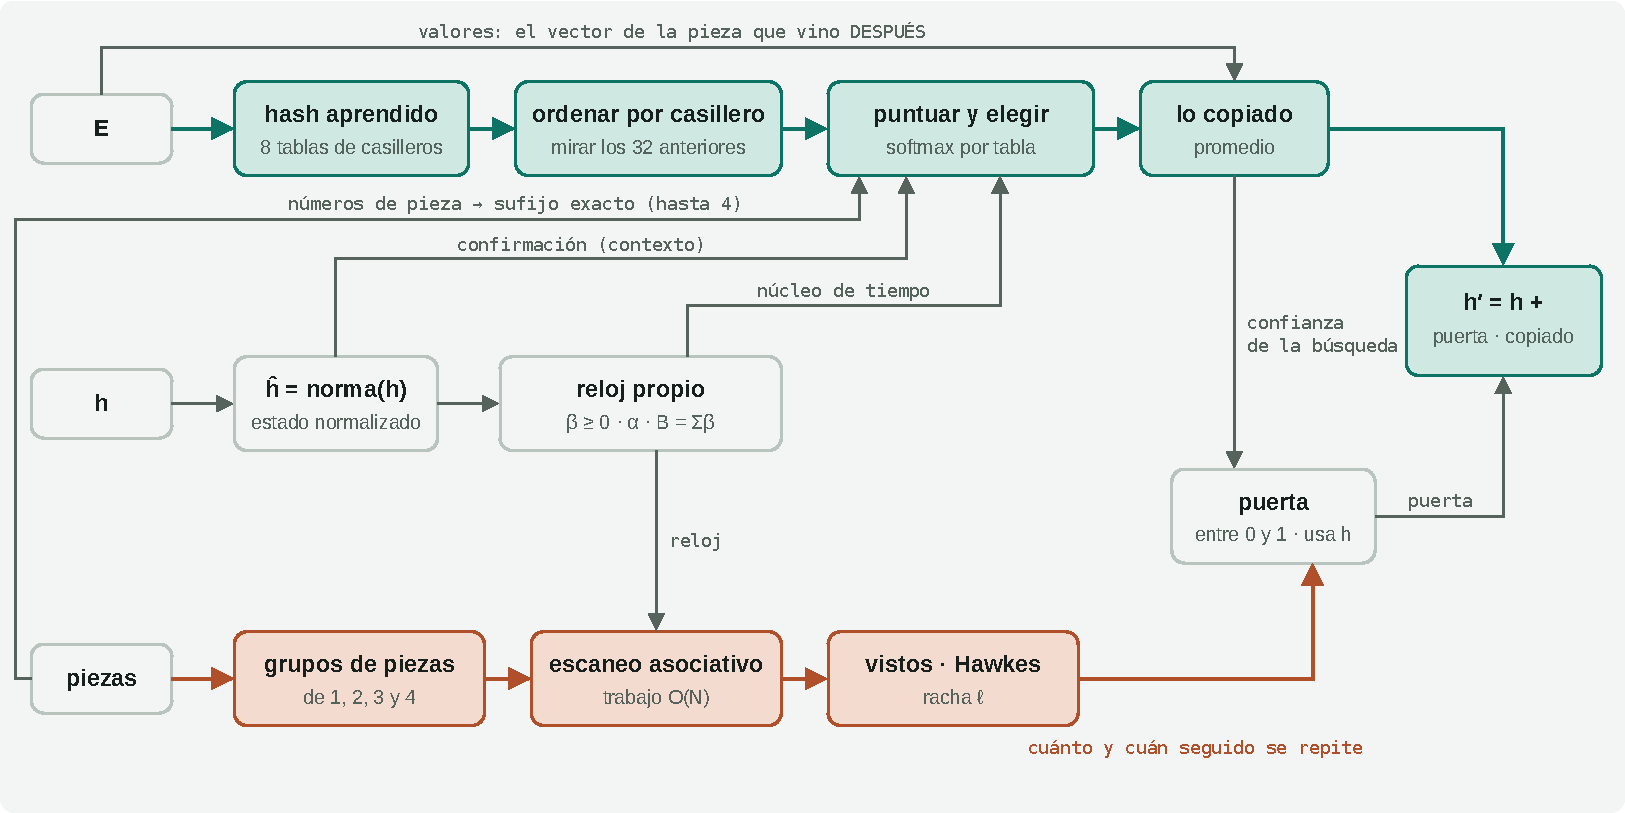
\includegraphics[width=0.78\linewidth]{capa_diagrama.pdf}
\caption{Dentro de una capa ASRN. Verde: \emph{dónde copiar} ---hash aprendido, orden por casillero, puntajes con un
softmax por tabla y el promedio de los valores copiados (el vector de la pieza \emph{siguiente}). Naranja: \emph{si
conviene copiar} ---los grupos de piezas y un escaneo asociativo dan la memoria de repetición (vistos, intensidad de
Hawkes y la racha, escrita $\ell$ en el diagrama y $\rho$ en el texto), que la puerta lee junto con la confianza de la
búsqueda. El reloj de tiempo propio, calculado a partir del estado normalizado, alimenta el núcleo de tiempo de los
puntajes y el escaneo.}
\label{fig:diagram}
\end{figure}

Las piezas $x_t\in\{0,\dots,V-1\}$ se convierten en vectores $E_t=\mathrm{Emb}[x_t]\in\mathbb{R}^d$. El modelo apila
\emph{bloques locales} causales, cada uno una convolución causal densa sobre la posición actual y las $k-1=3$ anteriores
seguida de un MLP de ancho $2d$,
\begin{equation}
h\leftarrow h+\GELU\!\big(\mathrm{Conv}^{\mathrm{causal}}_k(\LN_1 h)\big),\qquad
h\leftarrow h+W_2\,\GELU(W_1\LN_2 h),
\end{equation}
e inserta una capa ASRN cada dos bloques locales (después de los bloques $0,2,4,\dots$, salvo el último; una decisión
del desarrollo, ver \nolinkurl{history/}). La salida reutiliza la matriz del vocabulario,
$p(x_{t+1}\mid x_{\le t})=\softmax(\mathrm{Emb}\,\LN_f h_t)$; no hay tabla de posiciones, así que el orden entra por las
convoluciones y por el reloj. Una capa ASRN transforma el estado $h$ en
\begin{equation}
\boxed{\;h'_t=h_t+g_t\,W_o\,c_t\;}
\label{eq:layer}
\end{equation}
donde $c_t$ es \emph{lo copiado} (sección~\ref{sec:search}) y $g_t\in(0,1)$ es la \emph{puerta} de copia
(sección~\ref{sec:gate}); la figura~\ref{fig:diagram} muestra el flujo de datos. Tamaños por omisión: $T=8$ tablas de
$b=14$ bits (cuatro de ellas ven también la pieza anterior), $C=32$ candidatos, una confirmación de 16 dimensiones,
sufijos de hasta 4 piezas y grupos de 1 a 4 piezas.

\subsection{Reloj de tiempo propio}
\label{sec:clock}
Desde el estado normalizado $\hat h_t=\LN(h_t)$, cada capa calcula dos escalares por pieza:
\begin{equation}
\beta_t=\softplus(w_\beta^\top\hat h_t+b_\beta)\ge0,\qquad
\alpha_t=2\,\sigma(w_\alpha^\top\hat h_t+b_\alpha)\in(0,2),\qquad
B_t=\sum_{u\le t}\beta_u .
\label{eq:clock}
\end{equation}
$B_t$ es una reparametrización monótona del tiempo que depende de los datos: una pieza puede adelantar mucho el reloj
(un cambio de tema) o casi nada (dentro de una cita), y $\alpha_s$ dice cuán memorable es la aparición $s$. La memoria
se desvanece con el núcleo continuo
\begin{equation}
K_\kappa(t,s)=\alpha_s\,e^{-\kappa\,(B_t-B_s)},
\label{eq:kernel}
\end{equation}
un núcleo exponencial cuya distancia es tiempo propio y no número de piezas. Al empezar, $\beta_t=\alpha_t=1$, así que
el reloj cuenta piezas.

\subsection{Dónde copiar: búsqueda dispersa con hash}
\label{sec:search}
Dos MLP pequeños producen $T\cdot b$ coordenadas de hash por pieza; la mitad de las tablas ven también la pieza
anterior:
\begin{equation}
\varphi_t=\big[f_{\mathrm{word}}(E_t)\,;\,f_{\mathrm{ctx}}([E_t;E_{t-1}])\big]\in\mathbb{R}^{Tb},\qquad
\kappa_\tau(t)=\sum_{j=0}^{b-1}2^j\,\mathbf{1}[\varphi_{t,\tau,j}>0].
\end{equation}
En la tabla $\tau$, la pieza $t$ solo considera piezas anteriores de su propio casillero, a lo sumo las $C$ más
recientes: $\Nset_\tau(t)=\{$los $C$ mayores $s<t$ con $\kappa_\tau(s)=\kappa_\tau(t)\}$. Estos conjuntos salen de un
orden estable de las posiciones por casillero seguido de ventanas de $C$ preguntas contra $2C$ llaves, así que el
trabajo por pieza está acotado y la causalidad se cumple por construcción ($s<t$). Cada candidato recibe el puntaje
\begin{equation}
\mathrm{puntaje}_\tau(t,s)=
\underbrace{\frac{\langle\varphi_t,\varphi_s\rangle}{\sqrt{Tb}}}_{\text{similitud de hash}}
+\underbrace{\frac{\langle W_q\hat h_t,W_k\hat h_s\rangle}{\sqrt{16}}}_{\text{confirmación}}
+\underbrace{w^{\mathrm{suf}}_{\ell(t,s)}}_{\text{sufijo exacto}}
+\underbrace{\log\alpha_s-\frac{\gamma_\tau}{C}\,(B_t-B_s)}_{\text{núcleo de tiempo propio}},
\label{eq:score}
\end{equation}
donde $\ell(t,s)\in\{0,\dots,4\}$ es el largo del sufijo exacto común ($x_{t-1}=x_{s-1}$, $x_{t-2}=x_{s-2}$, \dots)
y $\gamma_\tau$ es una escala de tiempo aprendida por tabla. El último término es el logaritmo del
núcleo~\eqref{eq:kernel}: después del softmax es un núcleo de tiempo propio \emph{normalizado}. La capa copia la pieza
que vino \emph{después} de cada coincidencia:
\begin{equation}
a_\tau(t,s)=\softmax_{s\in\Nset_\tau(t)}\mathrm{puntaje}_\tau(t,s),\qquad
o_\tau(t)=\sum_{s\in\Nset_\tau(t)}a_\tau(t,s)\,W_vE_{s+1},\qquad
c_t=\frac{\sum_\tau o_\tau(t)}{\max(1,n_t)},
\end{equation}
con $n_t$ el número de tablas en las que $t$ tiene al menos un candidato ($o_\tau(t)=0$ si no tiene).

\subsection{Si conviene copiar: intensidad de Hawkes y racha de repetición}
\label{sec:repetition}
Para decidir si el texto está citando ahora, para el grupo de piezas que termina en $t$,
$G_n(t)=(x_{t-n+1},\dots,x_t)$, $n=1,\dots,4$, la capa calcula
\begin{align}
v_n(t)&=\mathbf{1}\big[\exists\,s<t:\,G_n(s)=G_n(t)\big] &&\text{(visto)}\\
\lambda_n(t)&=\sum_{s<t,\;G_n(s)=G_n(t)}\alpha_s\,e^{-\kappa_n(B_t-B_s)} &&\text{(intensidad de Hawkes)}\label{eq:hawkes}\\
\rho_t&=v_4(t)\,\big(e^{-\kappa_r\beta_t}\,\rho_{t-1}+1\big),\quad\rho_0=0 &&\text{(racha de repetición)}\label{eq:streak}
\end{align}
La ecuación~\eqref{eq:hawkes} es la intensidad de un proceso puntual autoexcitado~\cite{hawkes1971spectra} cuyos eventos
son las apariciones anteriores del mismo grupo de piezas, con el núcleo~\eqref{eq:kernel} \emph{sin normalizar} como
excitación. La racha $\rho_t$ mide el largo de la cita en curso. Las tasas $\kappa_n,\kappa_r>0$ se aprenden, empezando
en $\kappa_n=1/(C\,4^{\,n-1})$ y $\kappa_r=1/(8C)$: los grupos cortos olvidan rápido y los largos recuerdan más.

\subsection{La puerta y su respuesta no monótona}
\label{sec:gate}
\begin{equation}
g_t=\sigma\Big(w_g^\top h_t+w_{\mathrm{conf}}^\top\mathrm{conf}_t+b
+\sum_{n=1}^{4}w_n\,v_n(t)+\sum_{n=1}^{4}u_n\log\!\big(1+\lambda_n(t)\big)+f(\rho_t)\Big),
\end{equation}
donde $\mathrm{conf}_t$ son cuatro señales de confianza de la búsqueda (fracción de tablas con candidatos, mejor
puntaje, atención más alta, fracción de tablas de contexto con candidatos). La respuesta a la racha $f$ es lineal por
tramos sobre 16 nodos equiespaciados en $\log(1+\rho)$ hasta $\rho=256$ y constante más allá, parametrizada por
\emph{incrementos}:
\begin{equation}
z=\frac{\log(1+\rho)}{\Delta},\;\;\Delta=\frac{\log 257}{15},\;\;i=\lfloor z\rfloor,\qquad
f(\rho)=U_i+(z-i)(U_{i+1}-U_i),\qquad U_i=\sum_{j\le i}\delta_j .
\label{eq:response}
\end{equation}
Una respuesta monótona (por ejemplo $u\log(1+\rho)$) no puede expresar ``seguir hasta el largo normal de una cita y
entonces parar''; \eqref{eq:response} sí, y como los nodos que nunca ven datos reciben gradiente cero, la curva se
extiende \emph{plana} desde el último nodo observado. La motivación es el \emph{aliasing de estado}: una puerta que solo
ve señales que se saturan (vistos, sufijos de hasta 4 piezas) no distingue una cita de 5 piezas de una de 50.

\subsection{Un escaneo asociativo para todas las recurrencias}
\label{sec:scan}
Vistos, intensidades de Hawkes y racha son recurrencias lineales $S_i=a_iS_{i-1}+b_i$ con $a_i\in[0,1]$. Las funciones
afines se componen de forma asociativa, $(a_1,b_1)\circ(a_2,b_2)=(a_1a_2,\,a_2b_1+b_2)$, así que todas las posiciones se
resuelven en paralelo con un escaneo~\cite{blelloch1990prefix,martin2018parallelizing}: trabajo $O(N)$, profundidad
$O(\log N)$ y solo productos en $[0,1]$ y sumas (estable en fp32 y bf16). Un $a_i=0$ reinicia la recurrencia, así que
todos los segmentos se escanean a la vez. La intensidad de Hawkes reutiliza el orden de los vistos: en el orden por la
clave del grupo de piezas, la aparición anterior del mismo grupo es el elemento anterior y
\begin{equation}
S_i=a_i\,(S_{i-1}+\alpha_{i-1}),\qquad
a_i=\begin{cases}e^{-\kappa_n(B_i-B_{i-1})}&\text{mismo grupo que }i-1\\0&\text{si no.}\end{cases}
\label{eq:scan}
\end{equation}

\paragraph{Inicialización, complejidad y generación.} $w_\alpha$, $\gamma$, $w_n$, $u_n$, $\delta_j$,
$w^{\mathrm{suf}}$, $w_{\mathrm{conf}}$ y $W_q$ empiezan en cero y $\beta_t=\alpha_t=1$, así que una capa nueva calcula
lo que calculaba la capa más simple sin reloj, Hawkes ni racha. Por pieza y por tabla, ASRN puntúa una ventana de $2C$
llaves; solo el orden por casillero crece con $N$ ($O(N\log N)$ con un ordenamiento por comparación; en la GPU, un radix
sort con un número fijo de pasadas), y la memoria guardada es $O(N)$. Contada en CPU, una capa con $d=512$ cuesta 5.19 y
5.13 MFLOP por pieza con 1{,}024 y 16{,}384 piezas, contra 9.44 y 56.62 de la atención. Al escribir, cada tabla guarda,
por casillero, un anillo con las $C$ posiciones más recientes, que son justo las llaves a las que atiende una pieza
nueva, y cada clave de grupo de piezas lleva el reloj $B_u$ de su última aparición y $A=\lambda_n(u)+\alpha_u$, de modo
que $\lambda_n(t)=e^{-\kappa_n(B_t-B_u)}A$ y luego $A\leftarrow\lambda_n(t)+\alpha_t$, $B_u\leftarrow B_t$ (la
recurrencia~\eqref{eq:scan} llevada paso a paso); la racha es un solo número. Así, cada pieza nueva cuesta tiempo
$O(1)$, sin importar el contexto, mientras que la memoria sigue creciendo con el texto (los rasgos guardados de cada
posición, más anillos fijos de 17\,MiB por capa y por secuencia con los tamaños por omisión). Por omisión, los
candidatos se limitan a las posiciones cuya continuación está dentro del texto de inicio (\emph{memoria de lo ajeno}),
para que el modelo no quede atrapado copiando su propia salida, y una \emph{temperatura que conserva la cita} reescala
la distribución muestreada para que las piezas que continuarían un grupo de 4 ya visto conserven la probabilidad que les
da el propio modelo con $T=1$.

\subsection{Protecciones numéricas (ASRN 1.0)}
\label{sec:protections}
La versión 1.0 conserva la capa de v89 (\nolinkurl{asrn/nucleo.py}) y agrega una capa protegida con los mismos
parámetros (\nolinkurl{asrn/estable.py}), que se usa por omisión. Reproduce v89 salvo el redondeo en el régimen normal
($1.3\cdot10^{-7}$ en los logits) y cierra modos de falla de v89 encontrados por medición (A100, TF32 desactivado):
\begin{itemize}
\item \textbf{Máscara exacta.} v89 da a las llaves no válidas un puntaje finito, $-10^9$; si todos los puntajes válidos
  caen muy por debajo de ese valor, la masa del softmax se va a las llaves no válidas, entre ellas la propia pregunta,
  cuyo valor es la pieza siguiente. Con $\gamma=10^9$ el futuro cambió el pasado en $1.6\cdot10^{-2}$; normalizar solo
  sobre las llaves válidas lo vuelve 0.
\item \textbf{Reloj de 64 bits.} Un reloj en fp32 conoce el incremento $B_t-B_{t-1}$ solo con un error mediano de 2.2\%
  con $2^{20}$ piezas y se detiene en el 16\% de los pasos con $2^{24}$, y el término de tiempo de v89,
  $(\log\alpha_s+rB_s)-rB_t$, se cancela: correr el reloj $10^9$ cambia la salida en $8.8\cdot10^{-2}$. La capa estable
  acumula $B$ en fp64, lo pasa al kernel en dos partes fp32 y las resta antes de multiplicar por la tasa: corrimientos
  de $10^6$, $1.6\cdot10^7$ y $10^9$ cambian la salida en $5.5\cdot10^{-8}$ los tres, una diferencia de redondeo
  constante. Su proyección del reloj corre en fp32 de verdad: activar TF32 mueve el reloj sobre 65{,}536 piezas hasta
  1.98 unidades en v89 y $1.16\cdot10^{-10}$ en la capa estable.
\item \textbf{Topes}: $\beta\le10^4$, $\log\alpha\ge-30$, y la señal de mejor puntaje de la puerta recortada a
  $\pm10^4$.
\end{itemize}
Cuestan +7.5\% de tiempo y +5.2\% de memoria para una capa con 262{,}144 piezas (tabla~\ref{tab:layer}). Un segundo
grupo de protecciones cambia la función y está desactivado por omisión; no tuvo costo ni efecto medibles en la ablación.

\section{Experimentos}
\label{sec:experiments}

\paragraph{Montaje.} Todas las cifras en GPU salen de una ejecución de \nolinkurl{benchmarks/asrn_colab.ipynb} el 17 de
octubre de 2026 en una NVIDIA A100-SXM4-80GB en Google Colab (PyTorch 2.14.1, CUDA 13.0, autocast en bf16, huella del
código \texttt{5164e1f32513}); los resultados crudos están en \nolinkurl{results/banco_a100/}. ASRN es la capa estable
de la versión 1.0. Los modelos de comparación tienen el mismo ancho y casi el mismo número de parámetros:
\emph{Transformer++}, nuestra implementación de la receta de Llama~\cite{touvron2023llama} (RMSNorm, SwiGLU,
RoPE~\cite{su2024roformer}; el nombre sigue a~\cite{gu2023mamba}) con FlashAttention-2 a través de SDPA de PyTorch y sus
demás operaciones sin fusionar; \emph{Mamba-2}, el bloque original de \texttt{mamba\_ssm} 2.3.2 sin
\texttt{causal-conv1d} (su camino sin fusionar, así que las razones de velocidad de ASRN contra él son cotas
superiores); y \emph{RWKV-7}, el \texttt{RWKV7Model} original de flash-linear-attention 0.5.2~\cite{yang2024fla}. Todos
usan el mismo bucle de entrenamiento (AdamW, calentamiento y decaimiento coseno, recorte en 1, bf16, los mismos lotes
dentro de una semilla). Para cada modelo y tarea, la mejor de dos tasas de aprendizaje ($10^{-3}$, $3\cdot10^{-3}$) en
la semilla 0 según la métrica en el largo de entrenamiento (los empates van a la menor) se repite con las semillas 1 y
2; se informa media $\pm$ desviación estándar sobre 3 semillas. La tasa se elige con la misma evaluación que se informa,
y la comparación es a igual cantidad de datos, no a igual cómputo. Solo la velocidad de entrenamiento de ASRN y del
Transformer++ se midió también compilada.

\subsection{El cuello de botella: una capa de 1k a 262k piezas}
\label{sec:layer}

\begin{figure}[t]
\centering
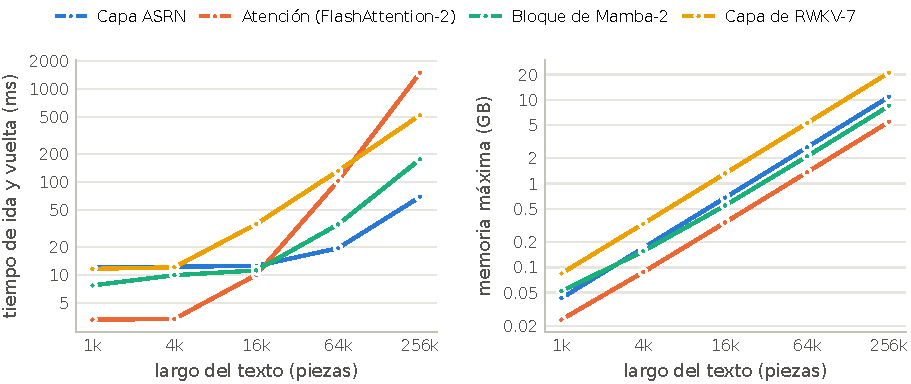
\includegraphics[width=0.94\linewidth]{capa.pdf}
\caption{Una capa, ida y vuelta, $d=512$, lote 1, bf16, sin compilar. Izquierda: tiempo; derecha: memoria máxima; los
dos ejes en escala logarítmica. La capa ASRN es la capa estable de la versión 1.0; la atención es FlashAttention-2 con
su RMSNorm; la unidad de Mamba-2 es su bloque entero (2.6$\times$ los parámetros de la capa ASRN); la capa de RWKV-7 es
la primera capa de un modelo de dos capas.}
\label{fig:layer}
\end{figure}

\begin{table}[t]
\centering\small
\setlength{\tabcolsep}{4.5pt}
\begin{tabular}{lrrrrrrr}
\toprule
& \multicolumn{3}{c}{tiempo (ms)} & \multicolumn{2}{c}{memoria máxima (GB)} & KiB/pieza & exponente \\
\cmidrule(lr){2-4}\cmidrule(lr){5-6}
Capa & 1{,}024 & 65{,}536 & 262{,}144 & 65{,}536 & 262{,}144 & con 262k & local\\
\midrule
ASRN 1.0 (capa estable) & 12.1 & \textbf{19.3} & \textbf{68.7} & 2.71 & 10.85 & 40 & 0.92\\
ASRN v89 (sin protecciones) & 12.0 & 18.0 & 64.0 & 2.58 & 10.31 & 38 & 0.91\\
Atención (FlashAttention-2) & \textbf{3.3} & 102.4 & 1{,}486.0 & \textbf{1.37} & \textbf{5.46} & \textbf{20} & 1.93\\
Bloque de Mamba-2 & 7.7 & 34.8 & 174.3 & 2.12 & 8.45 & 31 & 1.16\\
Capa de RWKV-7 & 11.6 & 131.1 & 519.4 & 5.28 & 21.10 & 79 & 0.99\\
\bottomrule
\end{tabular}
\caption{Una capa (el montaje de la figura~\ref{fig:layer}). Exponente local: pendiente log-log del tiempo entre
65{,}536 y 262{,}144 piezas (1 = lineal, 2 = cuadrático); el exponente de la memoria es 1.00 para todas. En
negrita: la mejor de las cuatro unidades.}
\label{tab:layer}
\end{table}

La atención tiene memoria lineal pero tiempo cuadrático (figura~\ref{fig:layer}, tabla~\ref{tab:layer}). El tiempo de
ASRN tiene un piso de unos 12\,ms hasta 16k piezas (muy probablemente el costo de lanzar kernels; no se perfiló) y
después crece de forma casi lineal. Por debajo de 16k piezas, ASRN está entre las unidades más lentas (la atención es
3.7$\times$ más rápida con 1k--4k piezas; RWKV-7 empata). Interpolando linealmente, ASRN pasa a la atención en
$\approx$17.8k piezas y al bloque de Mamba-2 en $\approx$20.2k (a RWKV-7 en $\approx$4.2k); con 262{,}144 piezas es
21.6$\times$ más rápida que la atención, 2.5$\times$ más rápida que el bloque de Mamba-2 (una unidad distinta y sin
fusionar; con modelos enteros la razón es 1.4--1.5) y 7.6$\times$ más rápida que RWKV-7. Su memoria es de unos 40\,KiB
por pieza, 2.0$\times$ la de la atención (RWKV-7 necesita 1.9$\times$ la de ASRN).

\subsection{Velocidad de entrenamiento y generación}
\label{sec:throughput}

\begin{figure}[t]
\centering
\begin{minipage}[c]{0.54\linewidth}
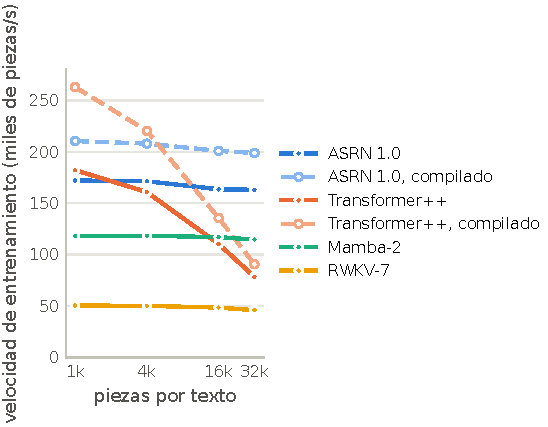
\includegraphics[width=\linewidth]{modelo.pdf}
\end{minipage}\hfill
\begin{minipage}[c]{0.43\linewidth}
\caption{Velocidad de entrenamiento de modelos de $\approx$50M parámetros (vocabulario 32{,}768, $d=512$) con
32{,}768 piezas por paso (lote $\times$ largo), bf16. Líneas continuas: sin compilar. Discontinuas, marcadores
huecos: ASRN compilado por partes y el Transformer++ con \texttt{torch.compile}; Mamba-2 y RWKV-7 no se
compilaron.}
\label{fig:throughput}
\end{minipage}
\end{figure}

Con el número de piezas por paso fijo y sin compilar, ASRN entrena a 172{,}065, 171{,}275, 163{,}503 y 163{,}023
piezas/s con 1k, 4k, 16k y 32k piezas por secuencia ($-5.3\%$; figura~\ref{fig:throughput}) y el Transformer++ de
182{,}116 a 78{,}400 ($-57\%$): el Transformer++ es 6\% más rápido con 1{,}024 piezas, y ASRN 1.07, 1.48 y
2.08$\times$ más rápido con 4k, 16k y 32k (cruce en $\approx$2.4k). ASRN es 1.40--1.46$\times$ más rápido que el
Mamba-2 sin fusionar y 3.38--3.55$\times$ más rápido que RWKV-7. Compilado por partes, ASRN entrena de 210{,}413 a
198{,}826 piezas/s (1.21--1.23$\times$ su velocidad sin compilar), y \texttt{torch.compile} acelera al Transformer++
1.44$\times$ con 1{,}024 piezas (262{,}909) y 1.15$\times$ con 32{,}768 (90{,}540): con ambos compilados, el cruce se
mueve a $\approx$5.4k piezas (el Transformer++ es 1.25$\times$ más rápido con 1{,}024 y ASRN 2.20$\times$ más rápido con
32{,}768). La memoria pico de ASRN (23.5\,GB) es 8\%, 11\% y 23\% menor que la del Transformer++, Mamba-2 y RWKV-7.

\paragraph{Generación.} Con lote 1 y la escritura $O(t)$ anterior, ASRN fue el que escribió más lento: unos 43\,ms por
pieza nueva (media 43.05 sobre contextos de 1k--64k piezas), contra 14.75 del Transformer++, 24.84 de Mamba-2 y 36.51 de
RWKV-7. El término $O(t)$ quedó escondido debajo de un costo fijo por pieza (pendiente ajustada de 3.0\,ns por pieza de
contexto, IC del 95\% $-25$ a 31), muy probablemente los lanzamientos de kernels (no se perfiló). La pasada del prefijo
sobre 65{,}536 piezas tarda 0.140\,s en ASRN, 0.387\,s en el Transformer++ y 0.139\,s en Mamba-2 (RWKV-7:
110.9--130.9\,s con cualquier largo, sobre todo compilación o autoajuste de kernels). La escritura $O(1)$ de la versión
1.0 da las mismas salidas (diferencia máxima de $2.2\cdot10^{-7}$ contra la pasada del texto entero), pero todavía no se
midió en la A100. En CPU (4 hilos, un modelo de 0.70M parámetros con 2 capas ASRN, lote 1;
\nolinkurl{results/escritura_cpu/}) se mantiene en 9.5--12.5\,ms por pieza nueva de 512 a 131{,}072 piezas de contexto
(pendiente de $-19$\,ns por pieza de contexto, IC del 95\% $-42$ a 3), mientras que la escritura $O(t)$ crece de 15.8 a
91.7\,ms (583\,ns, IC 537 a 629): 1.27$\times$ más rápida con 512 piezas y 9.7$\times$ con 131{,}072.

\subsection{Copia a larga distancia y recuperación asociativa}
\label{sec:copy}

\begin{figure}[t]
\centering
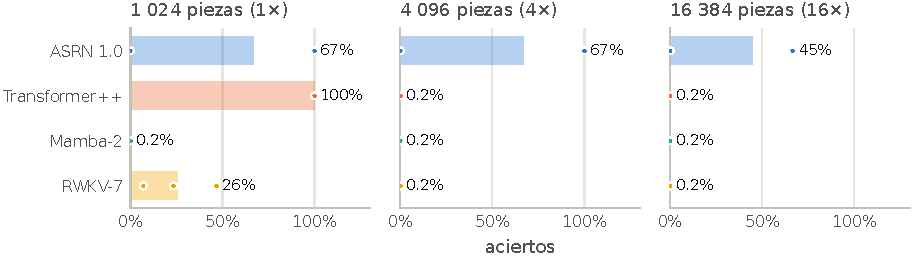
\includegraphics[width=0.92\linewidth]{copia.pdf}\\[3pt]
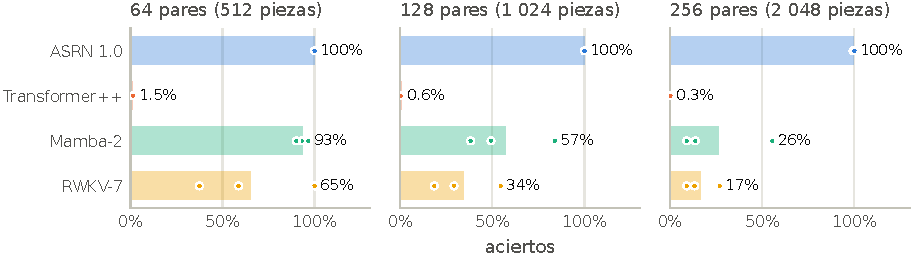
\includegraphics[width=0.92\linewidth]{mqar.pdf}
\caption{Arriba: aciertos al copiar con 1$\times$, 4$\times$ y 16$\times$ el largo de entrenamiento; un texto de
entrenamiento son 512 piezas al azar (vocabulario 512) seguidas de su repetición exacta, así que su segunda mitad pide
copiar desde 512 piezas atrás. Abajo: aciertos en MQAR~\cite{arora2023zoology} sobre los valores preguntados,
entrenado con 64 pares llave--valor en 512 piezas (vocabulario 8{,}192) y evaluado con 64, 128 y 256 pares en 512,
1{,}024 y 2{,}048 piezas. Barras y valores impresos: media de 3 semillas; puntos: cada semilla. La media de copia de
ASRN esconde dos semillas que aprendieron y una que se quedó en la meseta inicial (punto cerca de 0\%). Copia al azar:
0.2\%.}
\label{fig:copy}
\end{figure}

\begin{table}[t]
\centering\small
\setlength{\tabcolsep}{3pt}
\begin{tabular}{llrrrl}
\toprule
& & & & & pérdida $<1$\\
\textbf{Copia} & lr & 1{,}024 (1$\times$) & 4{,}096 (4$\times$) & 16{,}384 (16$\times$) & en el paso\\
\midrule
ASRN, semillas 0, 2 (salió) & $10^{-3}$ & 100.00, 100.00 & 99.99, 99.98 & 66.83, 66.49 & 1{,}000, 1{,}000\\
ASRN, semilla 1 (meseta) & & 0.10 & 0.15 & 0.18 & nunca\\
ASRN, media de 3 semillas & & $66.70\pm57.68$ & $66.71\pm57.64$ & $44.50\pm38.38$ & \\
Transformer++ & $10^{-3}$ & $100.00\pm0.00$ & $0.20\pm0.03$ & $0.22\pm0.01$ & 200 (todas las semillas)\\
Mamba-2 & $3\cdot10^{-3}$ & $0.19\pm0.07$ & $0.19\pm0.02$ & $0.21\pm0.01$ & nunca\\
RWKV-7 & $10^{-3}$ & $25.77\pm19.98$ & $0.25\pm0.02$ & $0.22\pm0.01$ & nunca\\
\midrule
\textbf{MQAR} & lr & 512 (64 pares) & 1{,}024 (128) & 2{,}048 (256) & 2{,}048, por semilla\\
\midrule
ASRN & $3\cdot10^{-3}$ & $\mathbf{99.99\pm0.02}$ & $\mathbf{99.99\pm0.01}$ & $\mathbf{99.75\pm0.43}$ &
100.00 / 99.25 / 99.99\\
Transformer++ & $3\cdot10^{-3}$ & $1.50\pm0.18$ & $0.56\pm0.18$ & $0.34\pm0.12$ & 0.31 / 0.46 / 0.24\\
Mamba-2 & $3\cdot10^{-3}$ & $93.20\pm3.27$ & $57.17\pm23.85$ & $26.09\pm25.55$ & 9.11 / 55.48 / 13.68\\
RWKV-7 & $10^{-3}$ & $65.43\pm31.76$ & $34.16\pm18.51$ & $16.51\pm9.34$ & 9.14 / 13.38 / 27.01\\
$p$ pareado contra Mamba-2 & & $p=0.070$ & $p=0.090$ & $p=0.039$ & \\
$p$ pareado contra RWKV-7 & & $p=0.20$ & $p=0.025$ & $p=0.0041$ & \\
\bottomrule
\end{tabular}
\caption{Aciertos (\%) en copia (2.5--2.9M parámetros) y en MQAR (4.4--4.9M), 2{,}000 pasos de entrenamiento, media
$\pm$ desviación estándar sobre 3 semillas (valores por semilla en el orden 0 / 1 / 2; pruebas $t$ pareadas sobre las
semillas). ASRN salió de la meseta inicial de la
copia en 2 de 3 semillas; la semilla 1 se quedó en ella los 2{,}000 pasos (pérdida final 6.232 $\approx\ln 511$). En la
corrida anterior en la A100 (sección~\ref{sec:replication}) las 3 semillas aprendieron la copia ($99.87\pm0.18$\% con
4$\times$).}
\label{tab:copy}
\end{table}

\paragraph{Copia.} Cuando ASRN sale de la meseta inicial, copia sin error en el largo de entrenamiento y casi sin error
con 4$\times$ (figura~\ref{fig:copy}, arriba; tabla~\ref{tab:copy}). Salir de ella en 2{,}000 pasos con $10^{-3}$ no
está garantizado (lo hicieron 5 de las 6 corridas de la base de las dos corridas en la A100), pero es un problema de
optimización y no de capacidad: con $3\cdot10^{-3}$, la semilla 0 salió de ella antes del paso 400 y llegó a 100\%,
99.99\% y 97.62\% (las dos tasas empataron al 100\% en el largo de entrenamiento, así que se eligió la menor). El
Transformer++ aprende la tarea al menos 4$\times$ antes que las semillas aprendidas de ASRN, pero cae al azar más allá
de su largo de entrenamiento, lo que estos datos no permiten atribuir a RoPE en distancias no
vistas~\cite{press2022alibi} en lugar de a una cabeza que aprendió un desplazamiento fijo de 511. Mamba-2 y RWKV-7 no
aprendieron dentro de este presupuesto, lo que no muestra que no puedan copiar: ASRN mismo se quedó en la misma meseta
durante unos 800 pasos.

\paragraph{MQAR.} ASRN mantiene su recuperación a medida que crece el número de pares (figura~\ref{fig:copy}, abajo),
al menos 99.25\% en cada semilla; eligió $3\cdot10^{-3}$ por un casi empate en la semilla 0 (100.00\% contra 99.97\%).
Mamba-2 cae de 93.2\% a 26.1\%, la caída que se espera de un estado de tamaño fijo~\cite{arora2023zoology}, confundida
con la extrapolación de largo y con una convergencia incompleta (pérdida final 0.33, 0.16 y 0.49); dos semillas de
RWKV-7 no convergieron (pérdida final 3.40 y 2.05). El Transformer++ no aprendió MQAR con ninguna de las dos tasas
(pérdida final 7.43--8.21, cerca de $\ln 4096=8.32$), una falla de este presupuesto o protocolo y no de la
atención~\cite{arora2023zoology}. Los resultados de los rivales no son estables entre corridas
(sección~\ref{sec:replication}); este MQAR, con llaves únicas seguidas de sus valores, está en el techo para ASRN.

\subsection{Modelado de lenguaje}
\label{sec:lm}

\begin{figure}[t]
\centering
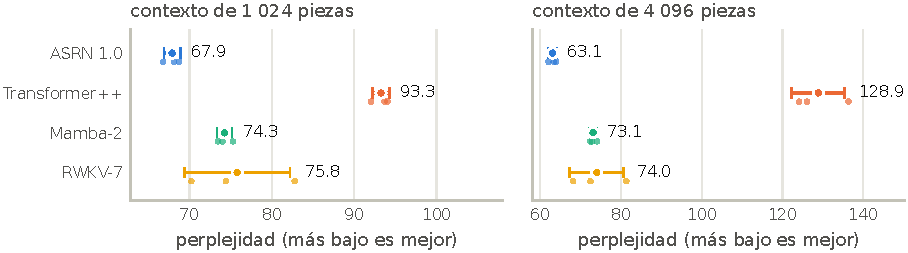
\includegraphics[width=0.94\linewidth]{texto.pdf}
\caption{Perplejidad de validación en WikiText-103 (más bajo es mejor) con 1{,}024 y 4{,}096 piezas de contexto,
después de 1{,}220 pasos de 16 secuencias de 1{,}024 piezas ($\approx$45M parámetros, $d=512$). Punto grande y raya:
media $\pm$ 1 desviación estándar de 3 semillas (media impresa); puntos chicos: cada semilla.}
\label{fig:text}
\end{figure}

\begin{table}[t]
\centering\small
\setlength{\tabcolsep}{4pt}
\begin{tabular}{lrlrrrl}
\toprule
& & & \multicolumn{2}{c}{perplejidad} & & $p$ pareado contra\\
\cmidrule(lr){4-5}
Modelo & Parám. & lr & contexto 1{,}024 & contexto 4{,}096 & 4k contra 1k & ASRN (1{,}024 / 4{,}096)\\
\midrule
ASRN 1.0 & 45.1M & $3\cdot10^{-3}$ & $\mathbf{67.91\pm1.00}$ & $\mathbf{63.08\pm0.97}$ & $-7.1\%$ & ---\\
Transformer++ & 44.4M & $10^{-3}$ & $93.27\pm1.07$ & $128.87\pm6.56$ & $+38.2\%$ & 0.002 / 0.003\\
Mamba-2 & 44.7M & $3\cdot10^{-3}$ & $74.25\pm0.92$ & $73.09\pm0.88$ & $-1.6\%$ & 0.008 / 0.003\\
RWKV-7 & 46.3M & $3\cdot10^{-3}$ & $75.81\pm6.39$ & $73.96\pm6.71$ & $-2.4\%$ & 0.13 / 0.084\\
\bottomrule
\end{tabular}
\caption{WikiText-103~\cite{merity2016pointer} (tokenizador de GPT-2), media $\pm$ desviación estándar sobre 3
semillas; prueba $t$ pareada sobre las semillas. La diferencia con RWKV-7 no es significativa.}
\label{tab:text}
\end{table}

Con los mismos datos y el mismo tamaño (figura~\ref{fig:text}, tabla~\ref{tab:text}), ASRN es el mejor en cada semilla
(66.81--68.76). Su ventaja sobre el Transformer++ y Mamba-2 es significativa con los dos largos de contexto; sobre
RWKV-7 no lo es: RWKV-7 varía mucho entre semillas (70.24--82.78) y queda detrás de ASRN en las tres, por 6.26, 3.43 y
14.02. Las salvedades pesan mucho: los modelos están lejos de converger (unas 0.44 posiciones de entrenamiento por
parámetro); las tasas quedan en los bordes de la grilla (con la misma $10^{-3}$ en la semilla 0 el orden fue Mamba-2
86.09, ASRN 89.55, Transformer++ 94.07); y WikiText-103 premia copiar, lo que favorece a la coincidencia exacta de
ASRN. Como historia del desarrollo, la quinta corrida de desarrollo (\nolinkurl{history/}), con otro protocolo y un
RWKV-7 \emph{reimplementado}, encontró a RWKV-7 claramente mejor ($47.87\pm0.15$ contra $57.02\pm0.32$ de la receta de
ASRN de v89). No se sostiene ninguna afirmación general de que ASRN supere a RWKV-7 en texto.

\subsection{Ablación: recuperación y regulación en tareas de copia pura}
\label{sec:ablation}

\begin{table}[t]
\centering\small
\begin{tabular}{llccrr}
\toprule
& & \multicolumn{2}{c}{copia: semillas} & copia 4$\times$, & MQAR\\
& & \multicolumn{2}{c}{que aprendieron} & peor & 2{,}048,\\
\cmidrule(lr){3-4}
& & esta & ambas & aprendida & media\\
Variante & Cambio & corrida & corridas & (\%) & (\%)\\
\midrule
\texttt{estable\_A} (base) & --- & 2 de 3 & 5 de 6 & 99.98 & 99.75\\
\texttt{estable\_AB} & + grupo B & 2 de 3 & 5 de 6 & 99.89 & 99.29\\
\texttt{sin\_puerta} & puerta fija en 1 & 2 de 3 & 4 de 6 & 99.98 & 99.94\\
\texttt{puerta\_sin\_senales} & la puerta solo ve $h$ & 3 de 3 & 6 de 6 & 99.98 & 99.50\\
\texttt{sin\_reloj} & $\beta=\alpha=1$, $\gamma=0$ & 2 de 3 & 4 de 6 & 99.98 & 99.95\\
\texttt{sin\_hawkes\_racha} & Hawkes y racha congelados & 3 de 3 & 6 de 6 & 99.98 & 99.53\\
\texttt{sin\_sufijo} & peso del sufijo congelado & 2 de 3 & 4 de 6 & 39.77 & 99.69\\
\texttt{sin\_confirmacion} & confirmación congelada & 3 de 3 & 6 de 6 & 99.93 & 99.88\\
\texttt{dos\_tablas} & 1 + 1 tablas & 1 de 3 & 2 de 6 & 99.67 & 98.99\\
\texttt{solo\_local} & sin capa ASRN & 0 de 3 & 0 de 6 & --- & 0.31\\
\texttt{mezcla\_lse} & mezcla por log-normalizador & 1 de 3 & 4 de 6 & 92.67 & 2.61\\
\bottomrule
\end{tabular}
\caption{Ablación: la capa estable con un componente quitado, 3 semillas, con las tasas elegidas para ASRN; la fila de
la base es la corrida de calidad de la sección~\ref{sec:copy}. ``Ambas corridas'' suma las 3 semillas de la corrida
anterior en la A100. Los componentes congelados se quedan en su valor inicial neutro, así que esas variantes calculan la
función base en el paso 0, con los mismos lotes; \texttt{dos\_tablas} usa 1 + 1 tablas en lugar de 4 + 4.}
\label{tab:ablation}
\end{table}

La copia es bimodal (una corrida o sale de la meseta inicial o se queda en el azar), así que la tabla~\ref{tab:ablation}
informa aparte las corridas que aprendieron. \textbf{La capa ASRN es lo que resuelve ambas tareas}: sin ella
(\texttt{solo\_local}, un campo receptivo de 13 piezas) las dos se quedan en el azar en todas las semillas de ambas
corridas en la A100. \textbf{En estas tareas el núcleo de recuperación basta y los mecanismos de regulación no son
intrusivos}: las corridas de copia que aprendieron de la base y de las variantes de regulación copian con 4$\times$ al
menos al 99.89\%, y sus medias de MQAR quedan entre 99.29\% y 99.95\%. \textbf{Tres semillas no pueden mostrar que
quitar la puerta, el reloj o el sufijo perjudique el aprendizaje}: la base misma se quedó en la meseta de la copia con
la semilla 1, igual que cinco variantes (en las dos corridas, 5 de 6 de la base contra 4 de 6 sin la puerta, el reloj o
el sufijo; Fisher $p=0.50$, unilateral). Menos tablas (2 de 6; $p=0.12$) y la corrida de \texttt{sin\_sufijo} que dio
87.02\% con 1$\times$ pero 39.77\% con 4$\times$ son solo sugerentes. La mezcla por log-normalizador, que salió primero
de la meseta de la copia en las 3 semillas de la corrida anterior, aquí lo hizo en 1 de 3, no aprende MQAR y cuesta
+62\% por corrida de copia; queda fuera de 1.0. Sin la puerta, sus señales, Hawkes y racha, o el reloj, una corrida de
copia tarda 17\%, 15\%, 8\% y 6\% menos; lo que estos mecanismos aportan se mide en la generación abierta.

\subsection{Aprender cuándo dejar de copiar}
\label{sec:quote}

% Cuerpo de la seccion "Aprender cuando dejar de copiar" (\input desde ASRN_Calvario_2026_es.tex).
% Fuentes: results/citas (CPU, la corrida principal), results/citas_a100 (su replicacion en la A100),
% docs/TECHNICAL_REPORT_es.md (seccion 7.2). Programa: benchmarks/experimento_citas.py.

Copia y MQAR no pueden poner a prueba los mecanismos de regulación: toda posición evaluada pide una copia, así que la
recuperación es todo lo que necesitan, y ahí la puerta, el reloj y las señales de Hawkes y de racha solo mostraron no
ser intrusivos (con ellos ASRN copia con 4$\times$ al 99.99\% y al 99.98\% en las 2 de 3 semillas que aprendieron y
llega a 99.75\% en MQAR con 4$\times$ los pares; sección~\ref{sec:ablation}). Su trabajo, decidir si copiar y cuándo
parar, importa al escribir libremente, así que su papel activo se prueba ahí, en un texto cuyas citas tienen un largo
acotado.

\paragraph{Montaje.} El texto son piezas al azar ($V=64$) en las que, con probabilidad 0.04 por posición, se cita un
trozo de las últimas 200 piezas de largo uniforme entre 6 y 12; en el texto real el 15.6\% de las piezas es
citado, y las rachas de grupos de 4 piezas ya vistos rara vez pasan de 9 piezas (lo hace el 0.9\%; la más larga es de
10). Se entrenan cinco modelos con la misma semilla, los mismos datos y la misma receta ($d=64$, dos bloques locales y
una capa ASRN, $L=256$, lote 16, tasa de aprendizaje $3\cdot10^{-3}$, 6{,}000 pasos con texto fresco): la capa completa
de 1.0; la capa sin las señales de Hawkes y de racha (congeladas en sus valores neutros); una puerta que solo ve el
estado oculto; sin puerta (fija en 1); y sin reloj ($\beta=\alpha=1$, $\gamma=0$). Cada uno escribe 128 piezas después
de inicios de 128 piezas de 64 textos de validación ($T=0.8$ con top-$k=40$ por omisión, y $T=1$; con y sin la memoria
de lo ajeno). Medimos la fracción de piezas escritas que cierran un grupo de 4 ya visto (\emph{citado}) y el largo de
las series seguidas de esas piezas (\emph{rachas}), juntando las semillas 0, 1 y 2. La corrida principal es en CPU
(\nolinkurl{results/citas/}); el banco de la A100 la repitió (\nolinkurl{results/citas_a100/}).

\begin{figure}[t]
\centering
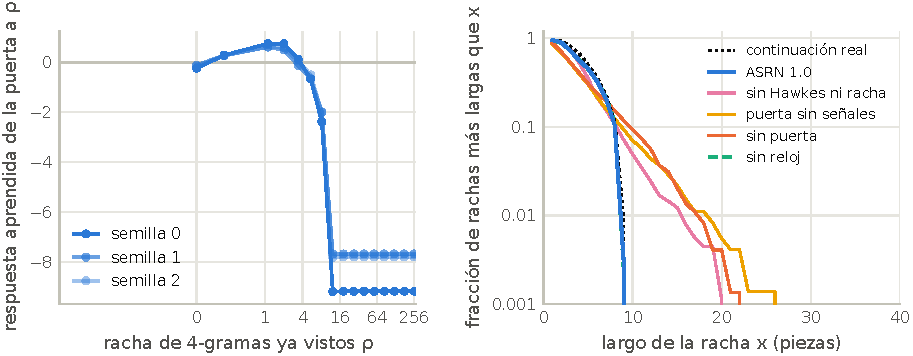
\includegraphics[width=0.94\linewidth]{citas.pdf}
\caption{Experimento de citas acotadas, corrida en CPU. Izquierda: la respuesta aprendida $f(\rho)$ de la puerta de la
capa completa a la racha de repetición $\rho$, tres semillas (eje logarítmico simétrico; nodos equiespaciados en
$\log(1+\rho)$ hasta 256). Derecha: fracción de las rachas escritas de más de $x$ piezas, juntando las tres semillas,
con el muestreo por omisión ($T=0.8$, top-$k=40$, memoria de lo ajeno activada); la curva sin el reloj casi coincide
con la de la capa completa.}
\label{fig:quote}
\end{figure}

\begin{table}[t]
\centering\small
\setlength{\tabcolsep}{3.3pt}
\begin{tabular}{lrrlrlrl}
\toprule
& \multicolumn{5}{c}{CPU (corrida principal)} & \multicolumn{2}{c}{replicación en la A100}\\
\cmidrule(lr){2-6}\cmidrule(lr){7-8}
& & & máx. & & & & máx.\\
Texto & citado & media & (por semilla) & $>9$ & pérdida val. & $>9$ & (por semilla)\\
\midrule
Continuación real & 15.6\% & 5.60 & 10 & 0.9\% & --- & 0.9\% & 10\\
\textbf{ASRN 1.0 (completa)} & \textbf{20.9\%} & \textbf{5.24} & \textbf{10} (9/10/10) & \textbf{0.3\%} &
3.7027--3.7056 & \textbf{0.3\%} & \textbf{10} (9/10/10)\\
sin Hawkes ni racha & 19.0\% & 5.22 & 21 (21/20/20) & 7.2\% & 3.7070--3.7079 & 7.9\% & 19 (17/15/19)\\
puerta sin señales & 13.9\% & 4.69 & 27 (17/23/27) & 9.3\% & 3.7290--3.7586 & 9.2\% & 39 (24/21/39)\\
sin puerta & 14.7\% & 4.91 & 23 (19/21/23) & 11.8\% & 3.7320--3.7396 & 12.0\% & 21 (21/20/20)\\
sin reloj & 20.2\% & 5.25 & 10 (10/10/9) & 0.2\% & 3.7042--3.7053 & 0.4\% & 10 (9/10/9)\\
\bottomrule
\end{tabular}
\caption{Escritura con el muestreo por omisión, semillas 0--2 juntas. \emph{Citado}: fracción de piezas escritas que
cierran un grupo de 4 ya visto; \emph{media}, \emph{máx.}: largo de las rachas; $>9$: porcentaje de rachas de más de 9
piezas; pérdida de validación: rango sobre las semillas.}
\label{tab:quote}
\end{table}

\paragraph{Qué aprende la puerta.} Solo con la pérdida de modelado de lenguaje, la puerta de la capa completa aprende
casi la misma respuesta en las tres semillas (figura~\ref{fig:quote}, izquierda): un empujón a copiar cuando empieza una
cita ($+0.62$ a $+0.76$ con $\rho\approx1$), negativo hacia $\rho\approx5$, y un freno fuerte desde $\rho\approx12$
($-7.7$ a $-9.2$), plano hasta $\rho=256$: un ``acantilado'' justo después de la racha más larga de los datos. La
respuesta sube y después baja, algo que una función monótona de la racha no puede expresar.

\paragraph{Efecto al escribir.} Con el muestreo por omisión, la capa completa escribe rachas como las del texto real
(tabla~\ref{tab:quote}, figura~\ref{fig:quote}, derecha): la más larga es de 10 y el 0.3\% pasa de 9 piezas. Sin las
señales de Hawkes y de racha, la racha más larga se duplica a 20--21 por semilla y el 7.2\% pasa de 9 piezas, aunque el
modelo cita casi lo mismo y su pérdida de validación es solo 0.002--0.005 más alta: el freno no se ve en la pérdida,
solo en lo que el modelo escribe. Con una puerta que no ve las señales, o sin puerta, el modelo cita menos, tampoco sabe
parar y su pérdida de validación empeora 0.03--0.05; sin el reloj escribe como la capa completa. El orden se mantiene
en todas las condiciones de muestreo (racha más larga por semilla de 9--10 para la capa completa, hasta 11 con la
temperatura que conserva la cita apagada, contra 15--36 de las tres variantes), y con $T=0.8$ apagar esa temperatura
sube la fracción citada de 20.9\% a 27.6\% y las rachas de más de 9 piezas de 0.3\% a 2.8\%.

\paragraph{Replicación en la A100.} Las mismas 5 variantes, 3 semillas y 6{,}000 pasos en la GPU reproducen el
resultado (tabla~\ref{tab:quote}, derecha): en todas las condiciones de muestreo, la racha más larga por semilla de la
capa completa es de 9--12 (12 solo con la memoria de lo ajeno desactivada y $T=0.8$) y sin el reloj de 9--10, contra
14--24 sin Hawkes ni racha, 15--39 con una puerta sin señales y 18--31 sin puerta. La pérdida de validación es
0.001--0.004 más alta sin Hawkes ni racha y 0.025--0.045 más alta con una puerta sin señales o sin puerta, y la
respuesta de la puerta tiene la misma forma ($+0.64$ a $+0.75$ con $\rho\approx1.1$, $-7.65$ a $-8.41$ desde
$\rho\approx12.3$).

\paragraph{Alcance.} Es una sola tarea sintética con tres semillas, $d=64$ y una capa ASRN. Quita juntas las señales de
Hawkes y de racha, y las entradas de la puerta en bloque, así que valida la puerta y sus señales de repetición, no cada
señal por separado. El reloj no tiene un efecto medible aquí, como se espera en una tarea sin cambios de tema. Cuán
seguido \emph{empieza} una cita no está calibrado (la temperatura que conserva la cita cubre solo su continuación): la
capa completa cita el 20.9--22.2\% de las piezas con $T=0.8$ y el 9.3--11.2\% con $T=1$ (21.8--24.2\% y 10.1--11.8\% en
la A100), contra 15.6\% en el texto real.


\subsection{Replicación entre dos corridas en la A100}
\label{sec:replication}

Una corrida anterior en la A100 (PyTorch 2.11, sin compilar, otra huella del código;
\nolinkurl{history/results/banco_a100_pt211/}), con el mismo protocolo, las mismas semillas y las mismas bibliotecas de
los rivales, sostiene las mismas conclusiones sobre velocidad, memoria, WikiText-103 y la recuperación de ASRN en MQAR
(una capa estable con 262{,}144 piezas: 66.2\,ms; WikiText-103 con 1{,}024 piezas: ASRN 67.78, Mamba-2 74.17, RWKV-7
72.35). Lo que varió: allí ASRN salió de la meseta de la copia en 3 de 3 semillas, y el MQAR de los rivales cambió mucho
(Mamba-2 con 2{,}048 piezas: $54.39\pm5.89$\% allí, $26.09\pm25.55$\% aquí; RWKV-7 con 512: $99.90\pm0.17$\% y
$65.43\pm31.76$\%), muy probablemente por kernels de GPU no deterministas que actúan sobre un entrenamiento sin
converger, mientras que ASRN se mantuvo en 96.4\% o más en cada semilla de ambas corridas.

\section{Trabajo relacionado}

Reformer~\cite{kitaev2020reformer} y el Routing Transformer~\cite{roy2021routing} también limitan cada pregunta a llaves
parecidas mediante hash o agrupamiento; el hash de ASRN es aprendido, su ventana es causal y está ordenada por recencia,
sus puntajes agregan sufijos exactos y un olvido en tiempo propio, sus valores son los vectores de las piezas
\emph{siguientes} (como en las cabezas de inducción~\cite{olsson2022induction}), y una puerta que conoce la repetición
controla la salida. La atención lineal~\cite{katharopoulos2020transformers}, los espacios de estados
selectivos~\cite{gu2023mamba,dao2024transformers} y RWKV-7~\cite{peng2025rwkv7} usan un estado de tamaño fijo con un
olvido que depende de los datos; el reloj de ASRN aplica en cambio un tiempo propio dependiente de los datos a
\emph{coincidencias exactas y dispersas}. Los modelos de estado fijo están limitados al copiar y
recordar~\cite{jelassi2024repeat,arora2023zoology}; nuestros resultados de MQAR coinciden con esto. Los mecanismos de
puntero y de copia~\cite{vinyals2015pointer,gu2016copynet,see2017pointergen,merity2016pointer} copian en la salida; ASRN
copia dentro de cada capa ASRN, sobre vectores. Los modelos de Hawkes neuronales~\cite{mei2017neural,zuo2020transformer}
predicen secuencias de eventos; en ASRN la intensidad de Hawkes~\cite{hawkes1971spectra} es un rasgo interno para la
puerta. Los escaneos asociativos~\cite{blelloch1990prefix} paralelizan las recurrencias
lineales~\cite{martin2018parallelizing,smith2023s5}.

\section{Limitaciones}
\label{sec:limitations}

\begin{itemize}
\item \textbf{Escala y protocolo.} 2.5--46M parámetros para la calidad y $\approx$50M para la velocidad, lejos de
  converger; dos tasas de aprendizaje elegidas con la misma evaluación que se informa; tres semillas; un solo corpus,
  que premia copiar; y un sesgo incorporado de coincidencia exacta, alineado con la copia y con MQAR. Los resultados de
  MQAR de los rivales variaron mucho entre dos corridas.
\item \textbf{Salida de la meseta de la copia.} La base salió de la meseta de la copia en 2 de 3 semillas aquí (5 de 6
  en las dos corridas en la A100), y 5 de las 24 corridas de las 8 variantes livianas de la ablación (la base,
  \texttt{estable\_AB} y las seis que quitan un componente) se quedaron en ella. La generalización con 16$\times$ varía
  con la semilla.
\item \textbf{La calidad en texto frente a RWKV-7 no está resuelta}: no es significativa ($p=0.13$), y una corrida de
  desarrollo anterior con un RWKV-7 reimplementado encontró el orden opuesto.
\item \textbf{Velocidad, memoria y modelos de referencia.} Por debajo de $\approx$18--20k piezas una capa ASRN es más
  lenta que la atención y que el bloque de Mamba-2, y con 1{,}024 piezas el Transformer++ entrena más rápido; ASRN
  necesita el doble de memoria que la atención y fue el que escribió más lento en la A100 (con la escritura $O(t)$; la
  $O(1)$ todavía no se midió ahí), y su memoria al escribir sigue creciendo con el texto. Mamba-2 corrió sin fusionar
  y sin compilar, solo ASRN y el Transformer++ se compilaron, y no se hizo ninguna comparación a igual cómputo.
\item \textbf{Mecanismos de regulación.} Su papel activo descansa en un solo experimento sintético (tres semillas,
  $d=64$, Hawkes y racha quitados juntos); el reloj no tuvo un efecto medible ahí, y su papel en los cambios de tema no
  está probado.
\end{itemize}

\section{Hoja de ruta / Trabajo futuro (v1.1+)}
\label{sec:future}

\textbf{La primera corrida de 100M parámetros}, con el kit listo para correr de un modelo de 103.5M parámetros sobre
FineWeb~\cite{penedo2024fineweb} en \nolinkurl{examples/train_100m/} y un barrido de largos de secuencia; \textbf{una
ablación a gran escala de los mecanismos de regulación} en corpus naturales con distractores y cambios de tema, con al
menos 5 semillas; \textbf{grillas de tasas de aprendizaje más anchas y presupuestos más largos} ($3\cdot10^{-4}$ y
$6\cdot10^{-4}$ para el Transformer++, $6\cdot10^{-3}$ para ASRN y Mamba-2, más pasos y semillas para la meseta de la
copia); \textbf{la generación en la GPU}: medir la escritura $O(1)$ en la A100 y recortar sus lanzamientos de kernels
por pieza (por ejemplo, con CUDA Graphs), que muy probablemente dominan ahí; \textbf{modelos de referencia compilados y
fusionados} (capa sola compilada, Mamba-2 y RWKV-7 compilados, Mamba-2 con \texttt{causal-conv1d}); y
\textbf{trabajo de kernels} que no cambia el modelo (una ventana deslizante persistente, un solo ordenamiento de grupos
de piezas compartido entre capas, un radix sort de 14 bits, un escaneo paralelo en la grilla).

\section{Conclusión}

ASRN elimina la dependencia del trabajo de entrenamiento por pieza respecto del largo del contexto para encontrar dónde
apareció antes el contexto actual y reutilizar lo que vino después; la versión 1.0 agrega protecciones numéricas. A la
escala probada, entrena a una velocidad casi independiente del largo de la secuencia, su capa es la unidad medida más
rápida más allá de unas 18--20k piezas, copia más allá de su largo de entrenamiento cuando sale de la meseta inicial (2
de 3 semillas) y mantiene la recuperación en MQAR con 4$\times$ los pares, y quedó primero en WikiText-103, de forma
significativa frente al Transformer++ y Mamba-2 pero no frente a RWKV-7. En la generación abierta controlada, su puerta
y sus señales de repetición aprenden, sin supervisión explícita, a detener las citas en el largo del texto real.

\section*{Reproducibilidad}
El código~\cite{calvario2026asrncode} es público (Apache 2.0) y está archivado junto con este preprint: el paquete
\texttt{asrn} (\nolinkurl{asrn/nucleo.py}, el núcleo de v89; \nolinkurl{asrn/estable.py}, la capa estable de la versión
1.0); las pruebas (57 del núcleo y 19 de la capa estable en \nolinkurl{tests/}, que la integración continua corre en
CPU; 7 verificaciones de GPU en \nolinkurl{tests/verificar_gpu.py}); un cuaderno para todas las secciones del banco en
la A100 (\nolinkurl{benchmarks/asrn_colab.ipynb}); el experimento de citas acotadas
(\nolinkurl{benchmarks/experimento_citas.py}); y la medición del tiempo de escritura
(\nolinkurl{benchmarks/medir_escritura.py}). Los resultados crudos están en \nolinkurl{results/banco_a100/},
\nolinkurl{results/citas/} y \nolinkurl{results/citas_a100/}, de los que \nolinkurl{paper/hacer_figuras.py} dibuja las
figuras, y en \nolinkurl{results/escritura_cpu/}. Los resultados de la A100 vienen de la huella del código
\texttt{5164e1f32513}, los primeros 12 dígitos hexadecimales del SHA-256 de las fuentes del paquete, de la raíz y del
banco, que el cuaderno imprime; la versión 1.0.0 solo difiere de ese código en la generación (la escritura $O(1)$ y sus
mediciones) y en los docstrings, y su pasada hacia adelante y sus gradientes son idénticos bit a bit. La historia del
desarrollo, que aquí no se usa como resultado, está en \nolinkurl{history/}; \nolinkurl{docs/TECHNICAL_REPORT_es.md} es
la versión larga de este preprint.

\section*{Contribuciones del autor}
Alexis Calvario concibió, diseñó, implementó y dirigió ASRN: la idea de una capa de copia que encuentra dónde apareció
antes el contexto actual, el reloj de tiempo propio, el uso de una intensidad de Hawkes y una racha para decidir cuándo
copiar, la implementación y los experimentos, y la dirección de cada versión (qué probar, qué resultados conservar y
cuáles descartar). Cada afirmación está respaldada por código que se puede correr y por las mediciones publicadas.

\section*{Licencia y cómo citar}
Este preprint (texto y figuras) se distribuye con licencia CC BY 4.0: se puede compartir y adaptar dando crédito al
autor. El código se distribuye con licencia Apache 2.0. Cítese como: A.~Calvario, \emph{ASRN: Adaptive Sparse
Recurrence Networks---linear-memory long-range copying with a learned proper-time clock and a Hawkes-gated copy gate},
preprint, Zenodo, 2026\ifx\zenododoi\empty\else, doi:\zenododoi\fi.

{\footnotesize\setlength{\bibsep}{1pt plus 1pt}
\bibliographystyle{unsrtnat}
\bibliography{referencias}}

\end{document}
